\documentclass[11pt]{article}

\usepackage{graphicx}
\usepackage{csquotes}
\usepackage{courier}
\setcounter{secnumdepth}{4}

\title{Locating a Target in Three Dimensions}
\author{Adam Yedidia}

\begin{document}

\maketitle
    
\section{Introduction}

\begin{figure}
\begin{center}
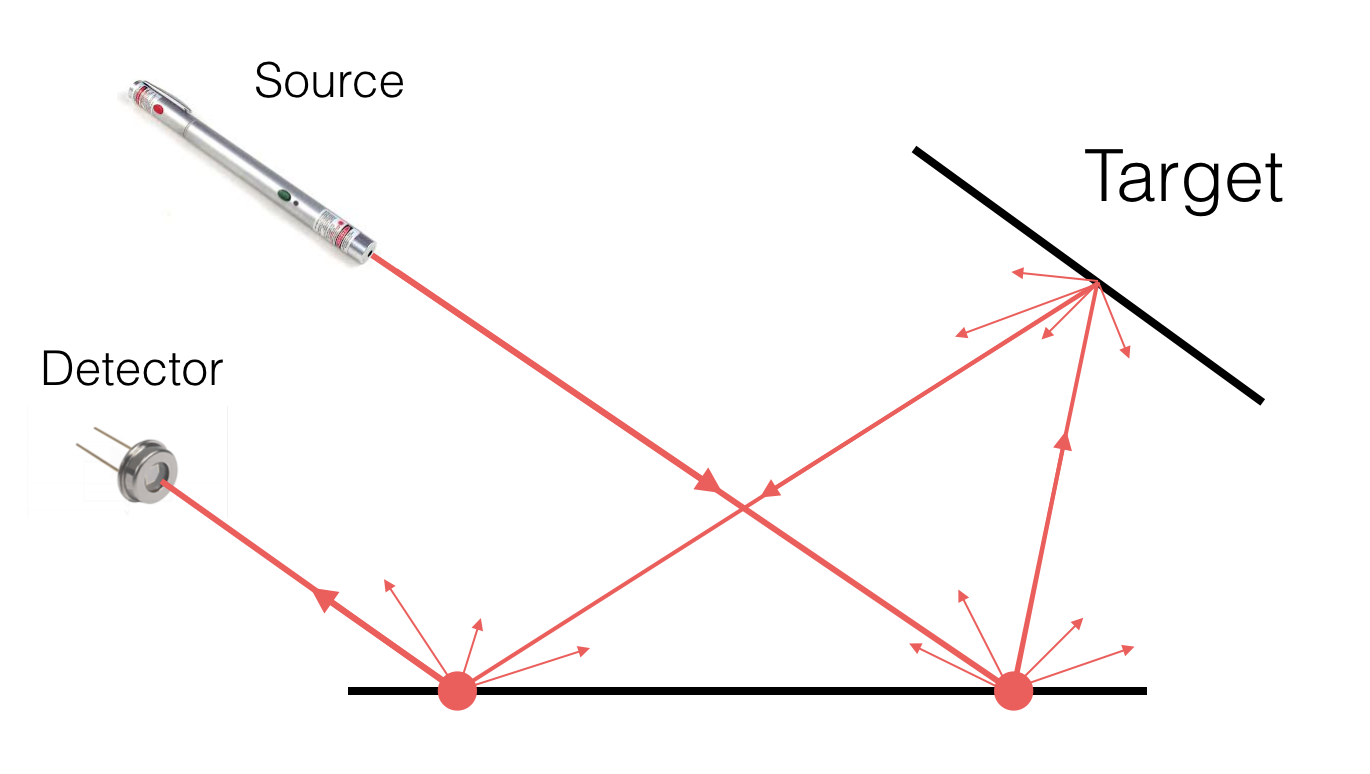
\includegraphics[scale=0.6]{figs/laser.png}
\caption{A view of the problem. Note that while this image is two-dimensional, the real problem I am concerned with is in three dimensions. \label{fig:laser}}
\end{center}
\end{figure}

This is an essay about using the light returns from a directional source and a directional detector\footnotemark~to locate a target in the three-bounce problem. For background on the three-bounce problem, see \emph{On the Localization of Objects Through the Emission and Detection of Light}.
\footnotetext{By a ``directional detector'' I mean a detector that only counts photons that are returning from a specific direction. I will use the term ``point detector'' to describe a detector that counts photons returning from \emph{any} direction (but that does not know the direction from which each photon came). It should be noted that a directional source directed at some point $p$ on a wall is equivalent to a point source of equal intensity directed at that same point $p$, up to glance factors; similarly, a directional detector directed at a point $q$ on a wall is equivalent to a point detector located at that same point $q$, up to glance factors. Therefore, for the sake of convenience in many future figures including Fig.~\ref{fig:twodthreed}, I represent the source and detector as simple point detectors at their locations on the wall; this is, of course, a simplification.}

This writeup is purely concerned with locating a flat surface-shaped target in three dimensions. Two-dimensional models are less interesting because they are qualitatively different: whereas the light bouncing off a three-dimensional target hits many points at once in such a way that all of them reach the detector at the same time, the light bouncing off a two-dimensional target hits only two points at the same time, which completely changes the form of the problem. See Fig.~\ref{fig:twodthreed} for a side-by-side comparison of the two-dimensional and three-dimensional versions of this problem.

\begin{figure}
\begin{center}
\centering
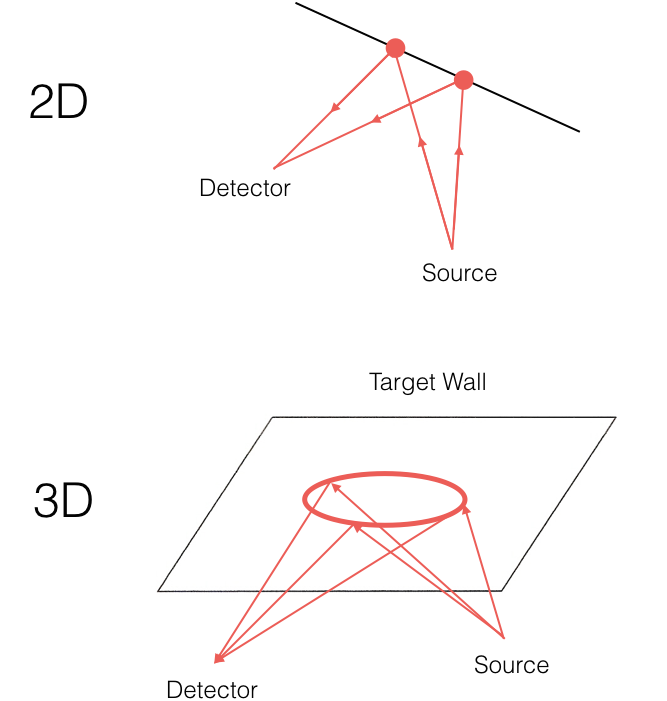
\includegraphics[scale=0.6]{figs/twodthreed.png}
\caption{A side-by-side comparison of a snapshot of the problem in two and in three dimensions. In both versions of the problem, the target is a surface, and the figures show the path taken by the light being received a short time after first light. In the two-dimensional case, the wall is a line, there are two points $p$ on the wall for which the total distance from the source to $p$ to the detector is equal to a given value. In the three-dimensional case, the wall is a plane, and there are infinitely many points $q$ on the wall for which the total distance from the source to $q$ to the detector is equal to a given value. For any given value, these points form an ellipse on the wall, as shown in the diagram. \label{fig:twodthreed}}
\end{center}
\end{figure}

As can be seen in Fig.~\ref{fig:twodthreed}, the points on the wall that mark the paths taken by the light from source to wall to detector form an ellipse. This is because they correspond to the points in three-dimensional space which both are equidistant to the source and the detector, and happen to lie on the plane of the wall. The points in three-dimensional space which are equidistant to two given points $p$ and $q$ form a prolate spheroid\footnotemark, with $p$ and $q$ as its foci; additionally, any cross-section of a prolate spheroid forms an ellipse.

\footnotetext{A \emph{prolate spheroid} is one way of extending the concept of the ellipse into three dimensions. Just as an ellipse can be defined by the lengths of its semi-major and semi-minor axes, so can an ellipsoid be defined by the lengths of its three axes, $a$, $b$, and $c$, with the equation $(\frac{x}{a})^2 + (\frac{y}{b})^2 + (\frac{z}{c})^2 = 1$. % TODO make sure that's actually true
If $a$, $b$, and $c$ are all different, that ellipsoid is known as a \emph{triaxial ellipsoid}. If $a = b$ and $c < a$ and $b$, that ellipsoid is called an \emph{oblate spheroid}, and has a shape like that of a Chinese bean pastry. If $a = b$ and $c > a$ and $b$, that ellipsoid is called a \emph{prolate spheroid}, and has a shape more like that of a football (but with curved points at the ends). Finally, of course, if $a = b = c$, the ellipsoid is a sphere. Although every circle has one focus, and every non-circular ellipse has two foci, not every non-spherical ellipsoid has two foci; indeed, only prolate spheroids have two foci, and only they can be described as the set of points in three dimensions equidistant from their two foci. Therefore, it is prolate spheroids that interest us in this problem, to the exclusion of other ellipsoids, because our interest is derived from the fact that we are interested in the set of points equidistant from the source and the detector.}

\section{A Forward Model} \label{sec:forwardmodel}

First, we will direct our interest towards the problem of efficiently computing the pattern of the light returns, as a function of the location of the target. As it turns out, computing the light returns from the target's location is a problem that can be solved in closed form.

Recall that the target is a plane. We therefore need three degrees of freedom to fully specify the plane's location and orientation. We can see this from the fact that the equation for a plane (using Cartesian coordinates) is $ax + by + cz = d$, with four degrees of freedom $a, b, c,$ and $d$, but with one redundant degree of freedom arising from the fact that the equation for the plane can be scaled without changing the plane's form. 

An alternate way of deriving the form of a plane from three specified values, which will turn out to be very convenient for this problem, is to specify the location of a single point, which is presumed to be the point of contact with the wall through which first light reaches the detector from the source. Because it's the point of \emph{first} contact, it is necessarily tangent to the prolate spheroid defined with the detector and source locations as its foci (that prolate spheroid describes the set of points that have the smallest total distance from the detector and source, that could still possibly intersect the target's plane). In this way, any plane can be described, with the exception of planes intersecting the line segment linking source and detector. These planes are of no interest to us in any case, because there would be no way to shoot a beam of light from the source to them to the detector without going \emph{through} the plane. (We presume the target plane is opaque.)

\subsection{Converting from First Contact Point to Plane}

\emph{Note: this section helps explain the} \texttt{getPlaneTangentTo} \emph{function in the source.}

Let's try converting from one of these schemes for describing planes to the other, for the sake of illustration. Imagine our source point (the point at which the directional source hits the reflecting wall) is at $(-l,0,0)$, and our detector point (the point at which the directional detector watches the reflecting wall) is at $(l,0,0)$. Therefore, we're likely to find it particularly useful to describe this plane in terms of what point on it is tangent to a prolate spheroid with foci $(-l,0,0)$ and $(l,0,0)$. This is because this point represents the point that the beam of first light heading from the source to the detector bounces off of. From now on, I will refer to this point as the \emph{point of first contact}. 

Let's suppose that that the plane is tangent to a prolate spheroid with those foci at the point $p = (x_p,y_p,z_p)$. We know that at that point, the partial derivatives of the equation for the spheroid and that for the plane should be equal. Call the semi-major and semi-minor axes of the prolate spheroid $A$ and $B$ respectively. If we'd like to describe this plane with a traditional Cartesian equation, $ax + by + cz = d$, then we know that the equation for the spheroid, $\frac{x^2}{A^2} + \frac{y^2}{B^2} + \frac{z^2}{B^2} = 1$. (The duplicate $B^2$ in the denominator is not a typo---recall that in a prolate spheroid, two of the axes must be the same length.)

If the partial derivatives with respect to each axis are to be equal at $p$, then we must have the equations:

\begin{equation}
a = \frac{2x_p}{A^2}
\end{equation}
\begin{equation}
b = \frac{2y_p}{B^2}
\end{equation}
\begin{equation}
c = \frac{2z_p}{B^2}
\end{equation}

Now that we know $a$, $b$, and $c$, we can solve for $d$ simply by using the equation of the plane:

\begin{equation}
d = ax + by + cz
\end{equation}

with the solutions for $a$, $b$, and $c$ above. This gives us the equation for the plane as a function of the point of first contact.

\subsection{Prolate Spheroidal Coordinates}

\emph{Note: this section helps explain the} \texttt{getPlaneTangentTo} \emph{and} \texttt{findSpotOnEggshell} \emph{functions in the source.}

From Wikipedia:

\begin{displayquote}

The most common definition of prolate spheroidal coordinates $(\mu, \nu, \phi)$ is

\begin{equation}
x = a \sinh \mu \sin \nu \cos \phi
\end{equation}
\begin{equation}
y = a \sinh \mu \sin \nu \sin \phi
\end{equation}
\begin{equation}
z = a \cosh \mu \cos \nu
\end{equation}

where $\mu$ is a non-negative real number and $\nu \in [0, \pi]$. The azimuthal angle $\phi$ belongs to the interval $[0, 2\pi]$.

\end{displayquote}

Fig.~\ref{fig:spheroidcoord} is a beautiful figure due to Wikipedia that illustrates the graphical meanings of $a, \mu, \nu,$ and $\phi$. 

\begin{figure}
\begin{center}
\centering
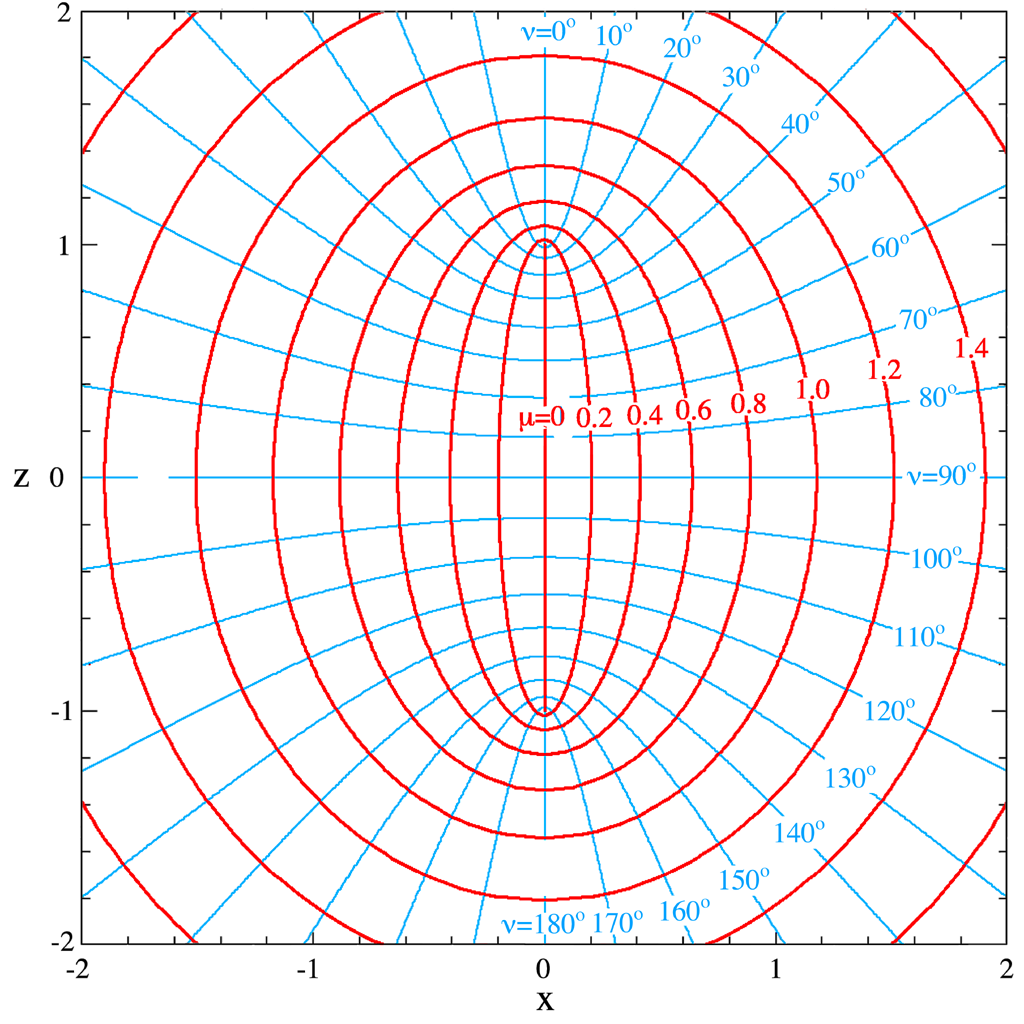
\includegraphics[scale=0.3]{figs/spheroidcoord.png}
\caption{Prolate spheroidal coordinates $\mu$ and $\nu$ for $a=1$. The lines of equal values of $\mu$ and $\nu$ are shown on the $x$-$z$ plane, i.e. for $\phi=0$. The surfaces of constant $\mu$ and $\nu$ are obtained by rotation about the $z$-axis, so that the diagram is valid for any plane containing the $z$-axis: i.e. for any $\phi$. Image and caption are due to Wikipedia, created by User:PAR (Own work). \label{fig:spheroidcoord}}
\end{center}
\end{figure}

Why are prolate spheroidal coordinates useful to this project? Because they form a useful lens through which to look at possible locations for the point of first contact. It is often useful to search over, for example, all points whose total distance from the source and the detector are equal to some constant. Prolate spheroidal coordinates simplify that process.

It's still not quite obvious how this works. From Fig.~\ref{fig:spheroidcoord}, we can see that varying $\nu$ takes us from one blue curve to the next, and is a little bit like the ``latitude'' of the point. Varying $\phi$ rotates the entire image, and is a little bit like the ``longitude'' of the point. You can't vary $a$---it's the distance from each focus to the center of the ellipsoid. Naturally, $a$ as used by Wikipedia is equivalent to $l$ from the previous section. Finally, varying $\mu$ is more confusing. Increasing $\mu$ seems to increase the size of the ellipsoid generated, like the radius of a sphere. It's not so simple, though, because the relationship between the ``diameter'' of the ellipsoid (the sum of the distances of any point on the ellipsoid from the two foci) isn't linear. 

Therefore, instead of reasoning about $\mu$, I use the variable $T$, which represents the time of first light (and, correspondingly, the aforementioned diameter of the ellipsoid). $T$ and $\mu$ have the following mathematical relationship:

\begin{equation}
\cosh(\mu) = \frac{T}{2l}
\end{equation}

In addition, we can derive the lengths of the semi-major and semi-minor axes of the prolate spheroid from $T$. The semi-major axis is the maximum distance of the center from any point on the spheroid. Naturally, this is equivalent to $\frac{T}{2}$. The semi-minor axis is the minimum distance of the center from any point on the spheroid. Because, on the ``equator'' of the spheroid (which is where the minimum distance from the foci is achieved), the points are equidistant from the two foci, we know that the distance from either focus to a point on the equator must be $\frac{T}{2}$. Thus, by the Pythagorean theorem, we can deduce the length of the semi-minor axis as well:

\begin{equation}
A = \frac{T}{2}
\end{equation}
\begin{equation}
B = \sqrt{\left(\frac{T}{2}\right)^2 - l^2}
\end{equation}

Thus, from this section, we can derive the semi-major and semi-minor axis lengths, which can be used to compute the equation for the plane as a function of the point of first contact as described in the previous section. Note, however, that when we compute the point of first contact in Cartesian coordinates as a function of its prolate spheroidal coordinates, we will need to rotate the axes with respect to Wikipedia's formulas, since in this document (and in the source), we take the foci to differ only on the $x$-axis, whereas on Wikipedia they differ only on the $z$-axis (as shown in Fig.~\ref{fig:spheroidcoord}).

\subsection{A Knowledge Inversion}

\emph{Note: this section helps explain the} \texttt{getParams} \emph{function in the source.}

So far, we have been thinking in terms of the target plane as an unknown quantity, and the locations of the source point and the detector point as known. But as is often the case, we can treat the problem as though the location of the target is known, and the locations of the source point and the detector point are unknown. 

In this spirit, we consider the problem from the opposite angle. Imagine that we know where the target plane is (without loss of generality, let's say it's at $z=0$). Now, just as we needed three values to locate the target plane previously, now we need three values to pinpoint the locations of the source and detector (up to translations and rotations, which will make no difference to the resulting time-series).

Without loss of generality, we can assume that both the source and detector are at $y=0$. In addition, we can assume that the source is at $x=0$ (but not the detector). This tells us that the source point, $p_s$, lies at $(0, 0, z_s)$. The detector point, $p_d$, lies at $(x_d, 0, z_d)$. Knowing $z_s, x_d$, and $z_d$, therefore, will allow us to pinpoint the source and detector.

How can we convert from our previous paradigm to this one? Well, we can take the locations of the source and detector, and compute their distance from the target plane. This gives us $z_s$ and $z_d$ respectively. Moreover, we can find the projections of each point onto the target plane, and find the distance between those projections, and that will give us $x_d$.

What does this achieve for us? Well, now, if we prefer, by starting from a hypothetical location for the target plane, we can convert to a hypothetical set of parameters $(z_s, x_d, z_d)$ and try to derive the time-series from that instead. No fundamental difference has occurred, and this step isn't strictly necessary, but I find it to make the math simpler.

\subsection{Computing the Time-Series}

\emph{Note: this section helps explain the} \texttt{approxFuncMaker} \emph{function in the source.}

Now that the setup is over, how do we actually go about computing the time-series? From here on out, we work under the most recent paradigm---that is, we assume that the target plane is at $z=0$, that the source point is at $(0, 0, z_s)$, and that the detector point is at $(x_d, 0, z_d)$

We begin by considering the horizon of possible ``bank shots.'' Excluding paths with more than one bounce, the only way for light to reach the detector point from the source point is via a bank shot. We can characterize the intensity of the incoming light as follows:

\begin{equation}
I(t) = \sum_{p \in P(t)} I_s(p)
\end{equation}

In the above, $I(t)$ refers to the intensity of the incoming light. This is what we are interested in calculating. $P(t)$ is the function that returns the set of paths whose length is $t$. Each of those paths has an associated individual intensity; this is what the $I_s(.)$ function computes.

Put another way, the total intensity at a given point in time is the sum of the intensities of all paths whose length is proportional to how much time has passed since the laser pulse. This is self-evident.

Now, what happens if we assume that at a given point in time, all paths have equal intensity? This convenient assumption removes the pesky sum from our equation:

\begin{equation}
I(t) = N_p(t) \cdot I_p(t)
\end{equation}

$N_p(t)$ refers to the total number of bank shots. $I_p(t)$ refers to the intensity per path. Computing the intensity function for a given $t$ will therefore proceed in two steps: computing $N_p(t)$, and computing $I_p(t)$.

\subsubsection{Computing $N_p(t)$}

What exactly is a ``path''? At this point, it is unavoidable that we have some discretization of space. Let's suppose that we subdivide two-dimensional space into little squares of side-length $\Delta x$. Counting the number of ``paths'' means counting the number of distinct ways to bounce across a number of different surfaces, choosing a different set of little squares to bounce off each time. So, as an example, if the light were to bounce off a $3\Delta x \times 3\Delta x$ surface, followed by a different off a $2\Delta x \times 5\Delta x$ surface, we might say that there were 90 total paths; 9 arising from the first surface, multiplied by 10 arising from the second. Of course, each path needn't contribute the same amount to the total intensity function; it is the work of the $I_p(t)$ term to take care of that issue.

Now we are ready to count the number of paths at a given point in time, $N_p(t)$. As a prelude to discussing how to compute $N_p(t)$, I will discuss how to compute $N_c(t)$: the \emph{total} number of bank shot paths with distance $t$ or less (rather than those with distance $t$). 

These bank shots must bounce off the target wall, which as a reminder lies at $z=0$ in our current paradigm. The set of acceptable bank shots (those with total distance $t$ or less) form a solid expanding prolate spheroid with foci the detector and source points. Naturally, the bank shots we care about are only those which intersect with the target wall. In other words, we are taking the cross-section of this prolate spheroid, at $z=0$. Any cross-section of a prolate spheroid yields an ellipse; we can therefore expect that $N_p(t)$ grows as the area of an ellipse.

Let us discuss this ellipse for a few moments. The area of any ellipse is given by the formula $\pi A B$, where $A$ is the semi-major axis of the ellipse (the maximum distance from the center of the ellipse to any point on the ellipse) and $B$ is the semi-minor axis of the ellipse (the minimum distance from the center of the ellipse to any point on the ellipse). This particular ellipse has its semi-major axis lying along the $y$-axis, and its minor axis lying parallel to the $x$-axis.

Why is this? Well, consider the points in the ellipse. In order for a point to lie within the ellipse, its total distance from the source and detector must not be too large. If only a small amount of time has passed since the first light has reached the detector from the source, the center of the ellipse also corresponds to the point on the target plane with the smallest total distance from the detector and source. This is a special point, and one worth naming; I'll call it the ``point of first contact,'' or $p_f = (x_f, 0, 0)$. 

Points on the target plane that deviate from $p_f$ are the ones that we are considering as candidates for being in the ellipse. Now consider the effect of a deviation from $p_f$ along the $x$-axis. The $x$-axis is the axis along which the source and the detector differ. When you deviate from $p_f$ a little along the $x$-axis, that brings you further from one of the detector or the source, but it brings you closer to the other. So deviating from $p_f$ a little along the $x$-axis won't increase your total from the detector and source by all that much.

Next consider the effect of a deviation from $p_f$ along the $y$-axis. The $y$-axis is the axis along which the source and the detector lie. When you deviate from $p_f$ a little along the $y$-axis, that brings you further from both the detector \emph{and} the source. Relative to deviations along the $x$-axis of equal magnitude, deviations along the $y$-axis will have a greater effect in terms of increasing your total distance from detector and source. Deviations along both the $x$- and $y$-axis of equal magnitude simultaneously will lie somewhere in between.

It follows, therefore, that the semi-major axis of the ellipse will lie along the $y$-axis, and that the semi-minor axis will lie parallel to the $x$-axis. Now, we can try to find $N_c(t)$.

\begin{equation}
N_c(t) = \frac{\pi A(t) B(t)}{(\Delta x)^2}
\end{equation}

Let $a_+$ and $a_-$ be the two possible deviations along the $x$ dimension from $p_f$ that the edge of the ellipse lies on (forwards and backwards). Let $t$ be the amount of time since first light. Let $T$ be the time of first light (and by the same token, the total distance from the source and detector to $p_f$). Thus, $t$ should be the distance of the source to $p_f$, plus the distance from $p_f$ to the detector, minus the time of first light. In other words:

\begin{equation}
t = \sqrt{(x_f+a_+)^2 + z_s^2} + \sqrt{(x_f+a_+-x_d)^2 + z_d^2} - T 
\end{equation}
\begin{equation}
t = \sqrt{(x_f-a_-)^2 + z_s^2} + \sqrt{(x_f+a_--x_d)^2 + z_d^2} - T
\end{equation}

Naturally, $p_f$ won't necessarily be the center of the ellipse---this will be the case if $t$ is not small compared to $T$ and $z_s \not= z_d$. If $p_f$ is not at the center of the ellipse, then $a_+ \not= a_-$. Of course, the ellipse will still have a semi-major axis---namely, that of the average between $a_+$ and $a_-$. Thus:

\begin{equation}
a = \frac{1}{2}(a_+ + a_-)
\end{equation}

At this point, we have three equations and three unknowns---$a_+$, $a_-$, and $a$. ($x_f$ is not unknown, because it is known to be the $x$-coordinate of the intersection point between the line including $(0,0,-z_s)$ and $(x_d, 0, z_d)$ and the $z=0$ plane---that is, $x_f = \frac{x_dz_s}{z_d + z_s}$).

When we solve for $a$, $a_+$, and $a_-$, we get a variety of solutions. We get the positive and negative versions of the true length of the semi-major axis $a$, of course---but we also get the difference between the distance from $p_f$ to one end of the ellipse and the distance from $p_f$ to the other. This yields the offset from $p_f$ to the true center of the ellipse---a value which grows, once again, as $t$ gets larger compared to $T$ and as $z_d$ differs more from $z_s$. We'll call the first kind of solution, which represents the length of the semi-major axis, $A$, and we'll represent the second kind of solution, which represents the how off-center the point of first light is, $a_o$. Note that the location of the of the center of the ellipse is now a known quantity---we'll call it $p_c$, and it lies at $(x_f + a_o, 0, 0)$.

Here are the formulas that come out of the solution of the above three equations:

\begin{equation}
A(t) = \frac{\sqrt{(t+T)^2((-(t+T)^2 + x_d^2 + z_d^2)^2 - 2z_s^2((t+T)^2-x_d^2+z_d^2)+ z_s^4)}}{2(t+T-x_d)(t+T+x_d)}
\end{equation}

\begin{equation}
a_o = \frac{(t+T)^2(x_d-2x_f) - x_d(x_d(x_d-2x_f) + z_d^2 - zs^2)}{2(t+T-x_d)(t+T+x_d)}
\end{equation}

We can find a formula for $B(t)$ in a very similar manner. $B(t)$ corresponds to the minimum distance from the center of ellipse to the edge of ellipse as a function of time. This axis will lie parallel to the $x$-axis, and corresponds to a change in $y$, since a change in $y$ makes the point further from both the source and the detector. We know that the amount of time $t$ that's passed since first light $T$ is equal to the distance from the source point $p_s$ to a point that is $b$ off center point along the $y$ dimension: $(x_c, b, 0)$ (where $x_c = x_f + a_o$), plus the distance from the center point to the detector point $p_d$. Thus, we have:

\begin{equation}
    t = \sqrt{x_c^2 + b^2 + z_s^2} + \sqrt{(x_c-x_d)^2 + b^2 + z_d^2} - T
\end{equation}

We know that $B(t)$, the length of the semi-minor axis as a function of time, is equal to $b$. Solving the above for $b$ gives us:

\begin{equation}
    \alpha = t^4 + 4t^3 T + T^4
\end{equation}
\begin{equation}
    \beta = 4tT(T^2 - 2x_c^2 + 2x_c x_d - x_d^2 - z_d^2 - z_s^2)
\end{equation}
\begin{equation}
    \gamma = (-2xx_d + x_d^2 + z_d^2 - z_s^2)^2
\end{equation}
\begin{equation}
    \delta = -2T^2(2x^2 - 2xx_d + x_d^2 + z_d^2 + z_s^2)
\end{equation}
\begin{equation}
    \epsilon = t^2(6T^2 - 2(2x^2 - 2xx_d+x_d^2 + z_d^2 + z_s^2))
\end{equation}
\begin{equation}
    B(t) = \frac{\sqrt{\alpha + \beta + \gamma + \delta + \epsilon}}{2(t+T)}
\end{equation}

So now we know $N_c(t) = \pi A(t) B(t)$, the total number of paths since first light. This is the integral of the number of paths at each point in time. Thus, we can retrieve the number of paths at a given point in time, $N_p(t)$, by taking the derivative with respect to time of $N_c(t)$:

\begin{equation}
    N_p(t) = \frac{d}{dt}N_c(t)
\end{equation}

Rather than take the mathematical derivative of the formula above derived, however, and get another formula many times larger, it is much simpler to take the numerical derivative. Therefore, we define here a small time increment: $\Delta t$.

Thus:

\begin{equation}
    N_p(t) = \frac{N_c(t + \Delta t) - N_c(t)}{\Delta t}
\end{equation}

\subsubsection{Computing $I_p(t)$} \label{sec:intensityperpath}

Recall that $I(t) = N_p(t) I_p(t)$. To compute the intensity function $I(t)$ given a time $t$ after first light, we must also know how to compute $I_p(t)$, the intensity per path.

$I_p(t)$ is assumed to be a constant. However, the intensity of a given path of course depends on where on the ellipse's edge the path reflects. That's a problem! Our assumption is wrong right off the bat. Of course, if we could make $I_p(t)$ the average path strength along the ellipse's edge, that would fix the issue. That's as hard to compute as the original integral equation, though.

Therefore, we are going to approximate. To compute our approximation $\hat{I_p}(t)$, we are going to average the intensity per path at the four points along the four axial points of the ellipse: $p_{a+} = (x_c + a, 0, 0)$, $p_{b+} = (x_c, b, 0)$, $p_{a-} = (x_c - a, 0, 0)$, and $p_{b-} = (x_c, -b, 0)$. We call the intensity per path coming from each of those points $I_{a+}$, $I_{b+}$, $I_{a-}$, and $I_{b-}$, respectively.

Thus: 

\begin{equation}
    \hat{I_p}(t) = \frac{1}{4}\left(I_{a+}(t) + I_{b+}(t) + I_{a-}(t) + I_{b-}(t)\right)
\end{equation}

\begin{figure}
\begin{center}
\centering
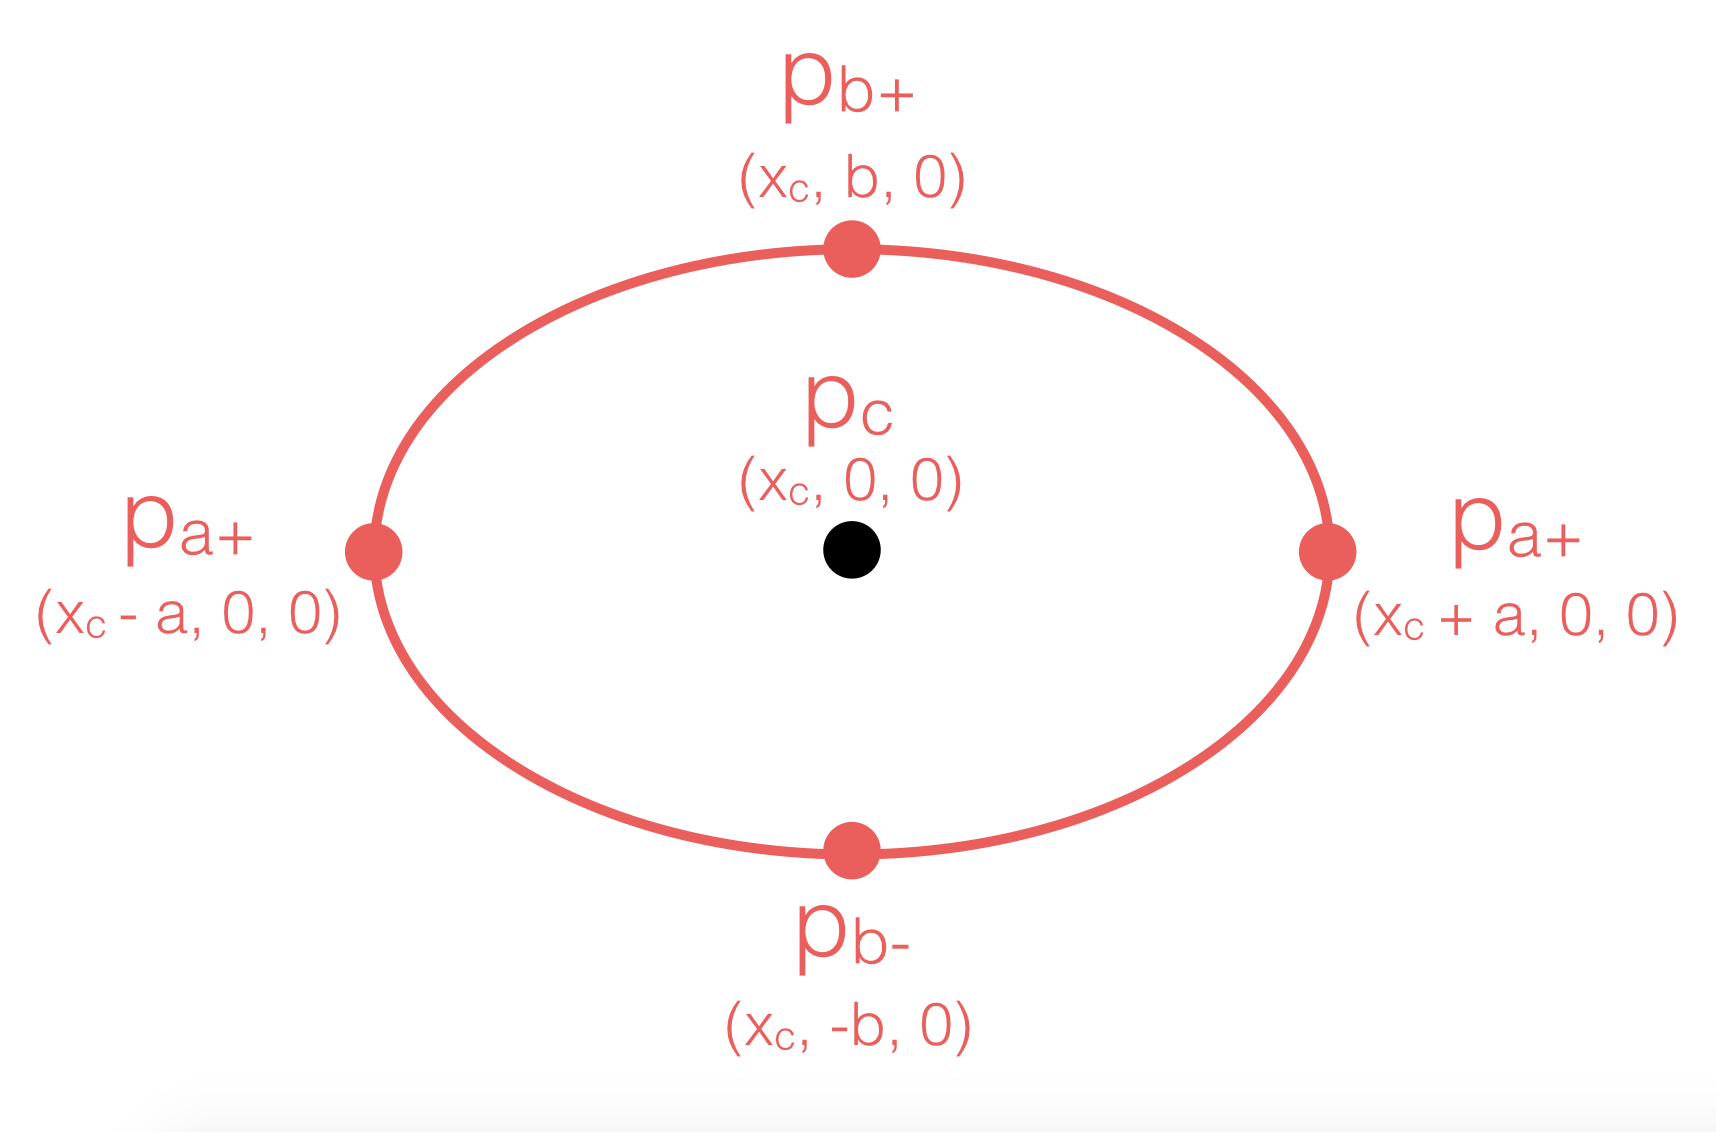
\includegraphics[scale=0.4]{figs/fourpoints.png}
\caption{The ellipse, with the four points over which we average shown in red. An exact measure of $I_p$ would average path intensity over the entire red ellipse; my approximation averages only over those four points. \label{fig:fourpoints}}
\end{center}
\end{figure}

How shall we compute the intensity per path at each of these points? Well, we know the location of each of the points. Recall from \emph{On the Localization of Objects Through the Emission and Detection of Light} that if light is being emitted in all directions from a point $(x, y, z)$, the fraction of that light that reaches a little square of side-length $\Delta x$ centered at $(0,0,0)$ and lying on the $z=0$ plane is: 

\begin{equation}
\frac{z (\Delta x)^2}{4\pi(x^2 + y^2 + z^2)^{\frac{3}{2}}}
\label{eq:wallz}
\end{equation}

More generally, if light is being emitted in all directions at point $(x_1, y_1, z_1)$, the fraction of that light that reaches point a little square of side length $\Delta x$ centered at $(x_2,y_2,z_2)$ and lying on a plane whose normal unit vector is $\vec{n}$ is:

\begin{equation}
    \left|\frac{(\Delta x)^2 (\{x_2-x_1, y_2-y_1, z_2-z_1\} \cdot \vec{n})}{4 \pi ((x_2-x_1)^2 + (y_2-y_1)^2 + (z_2-z_1)^2)^{\frac{3}{2}}}\right|
    \label{eq:wallgeneral}
\end{equation}

So let's recapitulate. There are going to be two legs in the journey from the source to the detector: one leg from the source to the target wall, and the other leg from the target wall to the detector. If we are interested in the intensity per path of bank shots off a given point $p_w$ on the target wall, then our intensity per path bouncing off that point, $I_p^{p_w}$, will look like this:

\begin{equation}
    I_p^{p_w} = I_p^{p_s \rightarrow p_w} \cdot I_p^{p_w \rightarrow p_d}
    \label{eq:intensityatpoint}
\end{equation}

How do we calculate $I_p^{p_s \rightarrow p_w}$? Well, we have our relevant equation in Eq.~\ref{eq:wallz}. Of course, in this case, light was not being emitted in all directions by the source point: because the source point is derived from a directional source colliding with a wall, light will be emitted in half of all directions. We know that $p_s$ is located at $(0, 0, z_s)$, and we suppose that $p_w$ is located at $(x_w, y_w, 0)$. This tells us:

\begin{equation}
    I_p^{p_s \rightarrow p_w} = \frac{z (\Delta x)^2}{2\pi(x_w^2 + y_w^2 + z_s^2)^{\frac{3}{2}}} 
    \label{eq:firstleg}
\end{equation}

As for the second leg, we can use Eq.~\ref{eq:wallgeneral} to help us compute it. Once again, light is only being emitted in all directions. We presume that the normal vector to the reflecting wall (\emph{not} the target wall) is $\vec{n_r}$. This tells us:

\begin{equation}
    I_p^{p_w \rightarrow p_d} = \left|\frac{(\Delta x)^2 (\{x_d-x_w, -y_w, z_d-z_w\} \cdot \vec{n_r})}{2 \pi ((x_d-x_w)^2 + y_w^2 + (z_d-z_w)^2)^{\frac{3}{2}}}\right|
    \label{eq:secondleg}
\end{equation}

Now that we know how to compute the intensity per path at a given point $p_w$, we can use it to compute the intensity per path at $p_{a+}$, $p_{b+}$, $p_{a-}$, and $p_{b-}$. This lets us compute our approximation for the intensity per path function, $\hat{I_p}(t)$, and from it our approximation for the intensity as a function of time, $\hat{I}(t)$. This, in sum, is our forward model: how we go from a collection of parameters $(T, \nu, \phi)$ to an intensity function that can be called for any value of $t$.

\section{Simulation}

\subsection{Method}

In order to verify the accuracy of the forward model, and get a sense for how much error the approximations described earlier introduce, there is a corresponding simulation to go with the forward model. I describe that simulation in this section.

The basic idea of the simulation is similar in spirit to the derivation of the forward model. It, too, relies on breaking down surfaces into many discrete points, and calculating total intensity from the individual contributions of each path.

We start with an empty histogram, representing the total intensity returning at each time interval $[t_i, t_{i+1}]$, where $t_{i+1} = t_i + \Delta t$. Then, for each discrete point on the target wall (each of which can alternately be thought of as a little square of side-length $\Delta x$), we compute the intensity of that path. We do this by borrowing some of the calculations described at the end of the previous section. In particular, for each point $p_w$ on the target wall, we use the last three equations described in the section to compute its contribution to the total intensity: Eqs.~\ref{eq:intensityatpoint},~\ref{eq:firstleg}, and~\ref{eq:secondleg}.

Having computed the intensity contribution of the path that bounces off the target wall at $p_w$, I insert it into the histogram at the appropriate time. To be specific, I compute the time of flight as follows:

\begin{equation}
t_w = ||\vec{p_s}-\vec{p_w}|| + ||\vec{p_w} - \vec{p_d}||
\end{equation}

I then find the bin in the histogram that corresponds to the interval which includes $t_w$, and increment that bin by $I_p^{p_w}$. Once I have done this for a sufficiently large set of points on the target wall---all points with $x_{\mathrm{min}} \le x_w \le x_{\mathrm{max}}$ and $y_{\mathrm{min}} \le y_w \le y_{\mathrm{max}}$, for some sufficiently small $x_{\mathrm{min}}$ and $y_{\mathrm{min}}$ and sufficiently large $x_{\mathrm{max}}$ and $y_{\mathrm{max}}$---the simulation is complete.

The runtime of this simulation is $O(\frac{(x_{\mathrm{max}} - x_{\mathrm{min}})(y_{\mathrm{max}} - y_{\mathrm{min}})}{(\Delta x)^2})$---potentially quite time-consuming if great precision is required. It is much slower than computing the time-series as described in Section~\ref{sec:forwardmodel}, which takes only a small amount of time, independent of the parameters chosen.

\subsection{Results}

\emph{Note: this section helps explain the} \texttt{doTwoPointPlaneExperimentWallDetect} \emph{function in the source.}

As can be seen from Fig.~\ref{fig:simresult}, the simulation matches the forward model very closely. The deviation in results right after first light is due to the fact that the intensity per path, $I_p(t)$, is computed by looking at the per-path intensity on the edge of ellipse. Normally, this is a very accurate approximation for small $\Delta t$, but very soon after first light, when the ellipse is expanding extremely rapidly (regardless of how small we make $\Delta t$), there will be plenty of relevant paths farther from the edge of the ellipse. This is a possible area for future work; perhaps a dual-regime forward model would perform better, with one regime concerning itself with the time very soon after first light and the other regime worrying about the time afterward.

\begin{figure}
\begin{center}
\centering
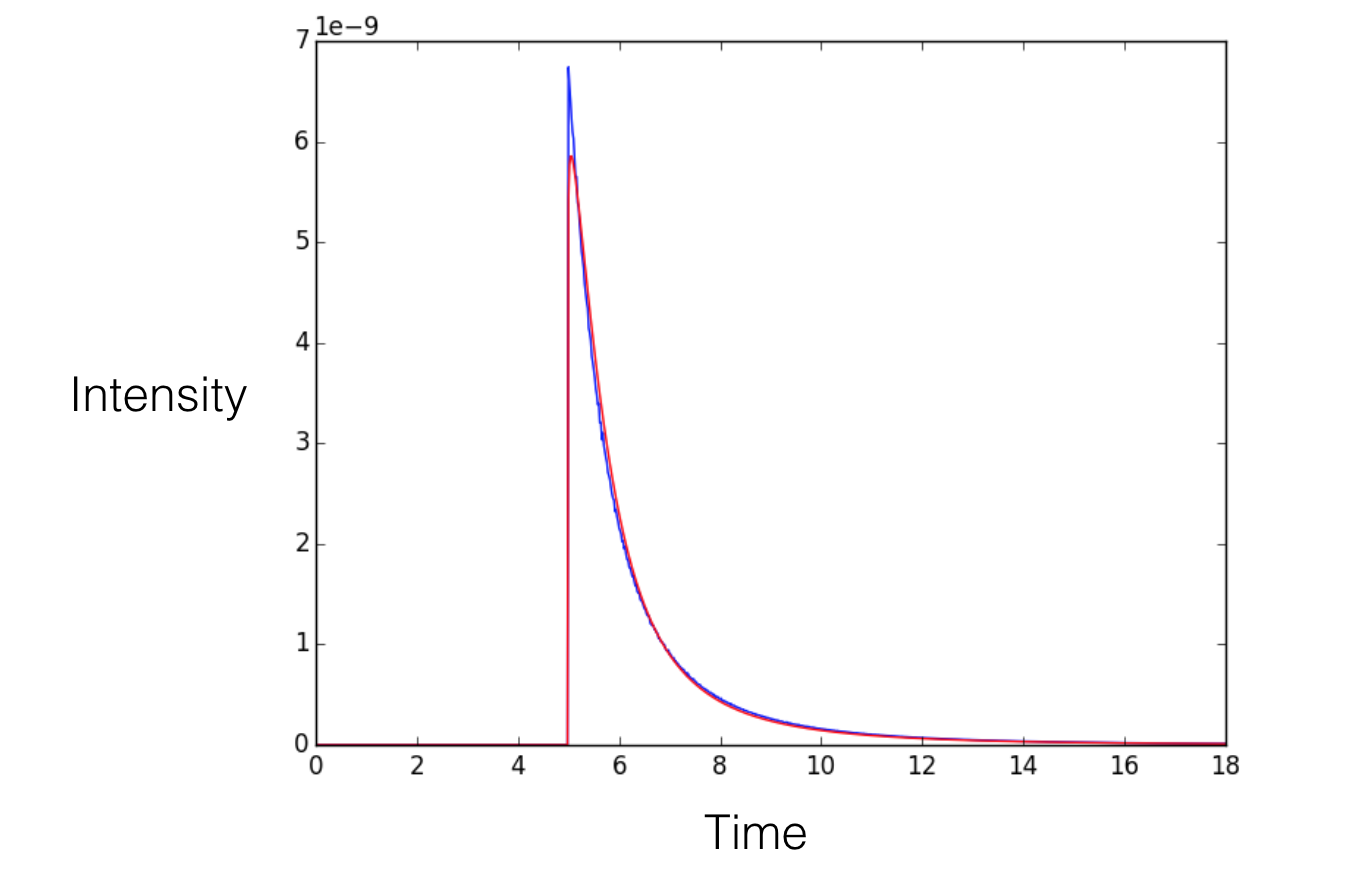
\includegraphics[scale=0.5]{figs/simresult.png}
\caption{A graph of intensity against time, from the simulation and from the forward model. The simulation is shown in blue and the forward model is shown in red. The parameters used for both the simulation and the forward model are: $\Delta x = 0.01$, $\Delta t = 0.02$, $z_s = 1$, $x_d = 3$, $z_d = 3$, $x_{\mathrm{min}} = -1.25$, $x_\mathrm{max} = 2.75$, $y_{\mathrm{min}} = -2$, $y_{\mathrm{max}} = 2$. \label{fig:simresult}}
\end{center}
\end{figure}

\section{Noise}

Up until this point, we have been considering only the idealized version of light, and observing the precise attenuation of light intensity from source to detector. This is reasonable assuming that the number of photons received by the detector is very large, and that the detector itself is perfect.

In practice, this ideal model may not fit reality all that well. First of all, no detector is perfect. Although modern-day detectors are very precise and are good enough to count individual photons, they will occasionally incorrectly report receiving a photon when none returned. And of course, this kind of noise may also be very important in situations where there are sources of illumination other than our laser pulse. I call this sort of noise \emph{background noise}.

In addition, after bouncing off walls three times, the light that returns to the detector is likely to be very faint. This means that few enough photons reach the detector that we can no longer assume the high-photon assumption that quantum effects are irrelevant; when few photons reach the detector, the fact that light returning from a laser pulse is a Poisson process becomes apparent. I call this sort of noise \emph{Poisson noise}.

\subsection{Background Noise}

\emph{Note: this section helps explain the} \texttt{addBackgroundNoise} \emph{function in the source.}

The way I model background noise is very simple---I move the entire ideal intensity distribution up by some noise constant $\eta$. This is equivalent to shining a light of constant intensity $\eta$ at the detector. This can both serve as a representation of sources of illumination other than the laser pulse, or as an erroneous detector which sometimes sees a returning photon when there was none.

\subsection{Poisson Noise}

\emph{Note: this section helps explain the} \texttt{poissonify} \emph{function in the source.}

In Section~\ref{sec:forwardmodel}, we discuss how to compute the attenuation of the light's intensity. The value that our forward-model function returns at each point in time is a fraction: the fraction of the total number of photons emitted by the source returning at that point in time.

In the photon-rich regime we implicitly assumed in that section, that's all there is to the story. To calculate how many photons will return at a given point in time, multiply the total number of photons $P$ emmitted by the fraction that return at any given point in time, and that's how many photons you will see at that point in time. 

In the more photon-sparse regime that we are introducing here, however, the story is more complicated. In fact, because the emission of photons is a Poisson process, the number of photons you'll calculate as being the number that return is actually the mean of a Poisson distribution. To get an exampe of what the actual time series might look like, you must sample from a Poisson distribution at each small time-interval.

\begin{figure}
\begin{center}
\centering
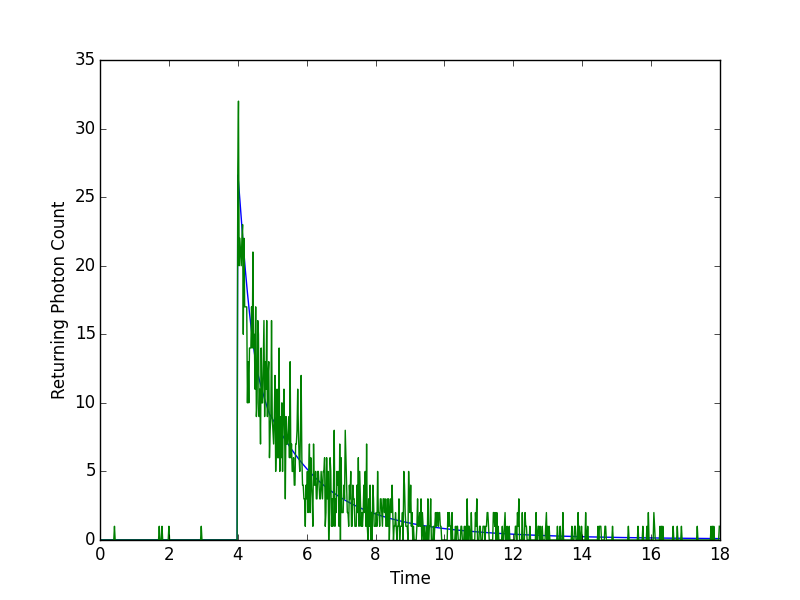
\includegraphics[scale=0.5]{figs/poisson.png}
\caption{A graph of intensity against time, with and without both sources of noise. In blue is intensity without noise, and in green is intensity with noise. The parameters are $d=1$, $T=4$, $\nu=\phi=0.785$, $\eta=1$, $P = 10^{10}$. \label{fig:poisson}}
\end{center}
\end{figure}

\section{Search}

Remember that I titled this write-up ``Locating a Target in Three Dimensions''! At last, we have gotten to the point where we can do some actual locating.

\subsection{Optimization Function}

\emph{Note: this section helps explain the} \texttt{logLikelihoodPoisson} \emph{function in the source.}

In order to search across possible locations for where the target wall could be, we need to know what we're looking for. In particular, we need to know what function to optimize that will be likeliest to give us an accurate estimate of the wall's location. 

In my search, I want to maximize the likelihood that the target wall is in the place that I decide is the correct one. Assuming that I don't think the target wall is particularly likelier to be in one place than another a priori, this approach is what will maximize the probability I chose the right spot.

What is the likelihood that the target wall is in a given spot? Well, to answer that, first we must consider the likelihood that the ``true'' light intensity is a given value at a given time.

Suppose that in the time interval $[t_i, t_i+\Delta t]$, we believe that the mean of the Poisson distribution is $l_i$. What is the likelihood that we observe $k_i$ photons arriving at the detector between $t_i$ and $t_i + \Delta t$?

Well, the Poisson distribution is given by

\begin{equation}
    P(k_i | l_i) = \frac{l_i^{k_i} e^{-l_i}}{k_i!} 
\end{equation}

So that would be the likelihood of observing $k$ photons conditioned on the mean of the Poisson distribution being $l$.

We can apply this technique to deduce the likelihood of getting the observations we got given that the target wall is in a given place. A set of observations means a number of photons for every little time-interval---and a corresponding likelihood for each one. To get the overall likelihood of the target wall being somewhere, we just need to multiply all the likelihoods together.

\begin{equation}
    P(\vec{k} | \vec{l}) = \prod_{i} \frac{l_i^{k_i} e^{-l_i}}{k_i!} 
\end{equation}

Of course, instead of maximizing the likelihood, we could just maximize the log of that quantity and get the same result.\footnotemark~This will be easier on the machine.

\footnotetext{For larger values of $k_i$ ($k_i > 10$ in the source) I use Sterling's approximation to compute $\log (k_i!)$: $\log(k_i!) \approx \log(\sqrt{2\pi}) + \frac{1}{2}\log(k_i) + k_i \log(k_i) - k$.}

\begin{equation}
    f(\vec{l}) = \log P(\vec{k} | \vec{l}) = \sum_{i} k_i\log(l_i) - l_i - \log(k_i!) 
\end{equation}

So there we have it! $f(\vec{l})$ is our optimization function. To find the ``fitness'' of a set of parameters $(T, \nu, \phi)$ given a set of observations $\vec{k}$, I use the forward model described in Section~\ref{sec:forwardmodel} to find the expected number of photons that we'd see if the wall was at $(T, \nu, \phi)$ under ideal circumstances, add on some background noise, and use the resulting vector $\vec{l}$ as the argument to $f(.)$.

\subsection{Search methods}

We're trying to find a triple $(T, \nu, \phi)$ that maximizes the function $f(.)$ from the previous section, and in so doing accurately describes where the wall is. Fortunately, we can infer $T$ right away (more or less) by just looking at the first time interval when a lot of photons showed up at once. In the source, I just take the middle of the first time interval in which at least 5 photons showed up to be $T$. This is somewhat hackety and of course doesn't generalize to extremely photon-sparse cases in which there is no instant where 5 photons show up at once; however, I haven't found the time-series to be at all useful beyond just providing the time-of-flight information in such extremely photon-sparse cases; I'll leave the study of that kind of regime to Justin. In the slightly more photon-rich regimes in which $T$ is immediately obvious, it helps the search a lot to be able to immediately infer it.

\subsubsection{Gradient Descent} 

My initial approach was a gradient descent over $\nu$ and $\phi$. Unfortunately, it seems like the space being searched over is non-convex, even in idealized photon-rich circumstances. 

An example gradient descent is shown in Fig.~\ref{fig:gradientdescent}.

\begin{figure}
\begin{center}
\centering
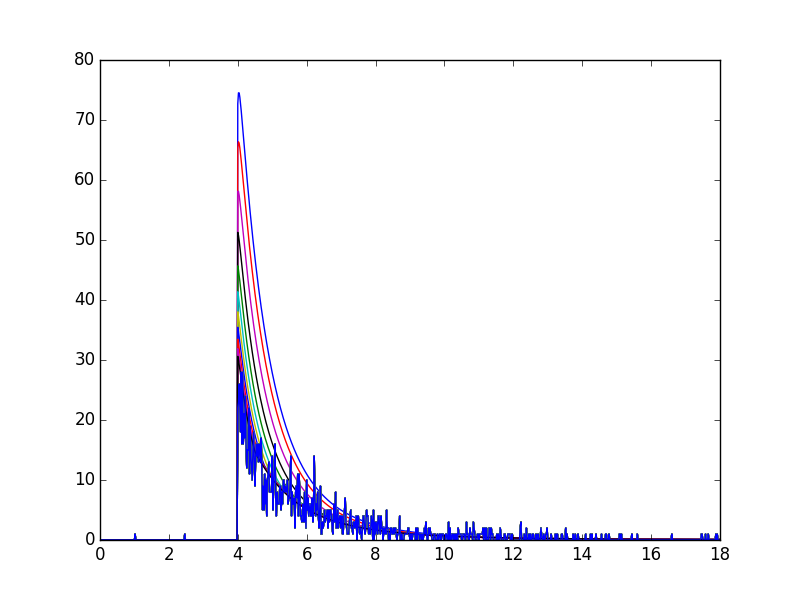
\includegraphics[scale=0.5]{figs/gradientdescent.png} %TODO label axes
\caption{A graphical representation of a gradient descent over $\nu$ and $\phi$, with the attempted parameters growing progressively closer to the truth. Unfortunately, the final set of parameters is still not the optimal solution. \label{fig:gradientdescent}}
\end{center}
\end{figure}

\subsubsection{Exhaustive Search}

Because we're searching over so few parameters, and computing $f(\vec{l})$ is relatively quick (taking time $O(\frac{t_{\mathrm{max}}}{\Delta t})$), it is simplest to just perform an exhaustive search over all pairs $(\nu, \phi)$ with $0 < \nu < \pi$ and $0 < \phi < \frac{\pi}{2}$ (by reflective symmetry across the $y=0$ plane, it is impossible to distinguish between the wall being at azimuthal angles $\phi$ versus $\pi - \phi$) to within some precision $\epsilon$.

The overall runtime of the exhaustive search is $O(\frac{t_{\mathrm{max}}}{\epsilon \Delta t})$---and for values of $\epsilon$ small enough that the inaccuracy introduced by $\epsilon$ is dwarfed by the inaccuracy introduced by noise for received photon counts around 1,000, running the exhaustive search takes about 10-20 minutes on my machine. Running this exhaustive search, for received photon counts of 1,000 or more, finds accurate values of $\nu$ and $\phi$ to within 0.01 radians. (Of course, a purely time-of-flight approach would have no idea about the values of $\nu$ and $\phi$!) For received photon counts more around 100, accuracy falls off sharply, and $\nu$ and $\phi$ can be pinpointed to within more like 0.1 or 0.2 radians.

\end{document}